\documentclass{article}
\usepackage{graphicx}
\usepackage{amsmath}
\usepackage{amssymb}
\usepackage{tikz}
\usetikzlibrary{automata, positioning, arrows}
\usepackage{booktabs}
\usepackage{float}
\usepackage{listings}
\usepackage{xcolor}
\usepackage{circuitikz}
\usepackage{karnaugh-map}
\usepackage{hyperref}
\usepackage[section]{placeins}

\title{Design and Implementation of a Moore Machine for "11011" Overlapping Sequence Detection}
\author{EE24BTECH11024 Abhimanyu Koushik\\EE24BTECH11002 Agamjot Singh\\IIT Hyderabad}
\date{\today}

\begin{document}

\maketitle

\section{Aim}
To design and implement a Moore machine-based sequence detector that identifies the pattern "11011" with overlapping capability using FSM theory, with sequence generation via Arduino and output visualization through an LED and oscilloscope.

\section{Apparatus}
\begin{itemize}
    \item Arduino Uno
    \item 7474 ICs (D flip-flops) - 2 pieces
    \item 3-Input AND Gate IC (7441)
    \item 2-Input OR Gate IC (7432)
    \item Breadboard and connecting wires
    \item LED and appropriate resistors (220 $\Omega$)
    \item Cathode Ray Oscilloscope (CRO)
    \item 5V DC power supply
\end{itemize}

\section{Theory}

\subsection{D Flip-Flops and Sequential Logic}
The D flip-flop is a fundamental memory element in sequential logic. Its operation can be described by:
\[
Q(t+1) = D(t)
\]
where the next state directly reflects the data input at each clock edge.

\subsection{State Diagram}
The Moore machine state diagram comprises six states:
\begin{itemize}
    \item \textbf{$S_0$}: Initial state (no bits detected)
    \item \textbf{$S_1$}: Detected ``1''
    \item \textbf{$S_2$}: Detected ``11''
    \item \textbf{$S_3$}: Detected ``110''
    \item \textbf{$S_4$}: Detected ``1101''
    \item \textbf{$S_5$}: Detected ``11011'' (complete sequence)
\end{itemize}
Transitions between states are triggered by the input bits, and only state $S_5$ produces an output 1.

\begin{figure}[!ht]
\centering
\resizebox{1\textwidth}{!}{%
\begin{circuitikz}
\tikzstyle{every node}=[font=\Huge]
\draw  (7.5,14.5) circle (1.75cm);
\draw  (17.5,14.5) circle (1.75cm);
\draw  (0,7) circle (1.75cm);
\draw  (7.5,-0.5) circle (1.75cm);
\draw  (17.5,-0.5) circle (1.75cm);
\draw  (25,7) circle (1.75cm);
\node [font=\Huge] at (7.5,15) {$S_0$};
\draw [->, >=Stealth] (10,13.75) -- (15,13.75);
\draw [->, >=Stealth] (19.25,12.75) -- (23.25,8.75);
\draw [->, >=Stealth] (23.25,5.25) -- (19.5,1.25);
\draw [->, >=Stealth] (15,-0.5) -- (10,-0.5);
\draw [->, >=Stealth] (5.75,1.25) -- (2,5);
\draw [->, >=Stealth] (2.5,7) -- (22.5,7);
\draw [->, >=Stealth] (2.25,6) -- (16,1);
\draw [->, >=Stealth] (17,1.75) -- (9,12.75);
\draw [->, >=Stealth] (15,15) -- (10,15);
\draw [->, >=Stealth] (5.25,-0.25) .. controls (-7.25,1) and (-7.25,13.5) .. (5.25,14.75) ;
\draw [->, >=Stealth] (6,16.25) .. controls (5.25,18.25) and (7.5,18.75) .. (8,16.75) ;
\node [font=\Huge] at (7,17.5) {};
\draw [->, >=Stealth] (27,8.25) .. controls (29.5,8) and (29.5,5.75) .. (27,5.75) ;
\node [font=\Huge] at (7.5,14) {0};
\node [font=\Huge] at (12.5,12.75) {1};
\node [font=\Huge] at (22,11.25) {1};
\node [font=\Huge] at (29.5,7) {1};
\node [font=\Huge] at (9.5,7.75) {1};
\node [font=\Huge] at (9,2.75) {0};
\node [font=\Huge] at (-5,7.25) {0};
\node [font=\Huge] at (13,-1.25) {1};
\node [font=\Huge] at (22.5,2.75) {0};
\node [font=\Huge] at (15.5,5.25) {0};
\node [font=\Huge] at (17.5,15) {$S_1$};
\node [font=\Huge] at (17.5,14) {0};
\node [font=\Huge] at (25,7.5) {$S_2$};
\node [font=\Huge] at (25,6.5) {0};
\node [font=\Huge] at (17.5,0) {$S_3$};
\node [font=\Huge] at (17.5,-1) {0};
\node [font=\Huge] at (7.5,0) {$S_4$};
\node [font=\Huge] at (7.5,-1) {0};
\node [font=\Huge] at (0,7.5) {$S_5$};
\node [font=\Huge] at (0,6.5) {1};
\node [font=\Huge] at (6.25,18.5) {0};
\node [font=\Huge] at (12.5,15.75) {0};
\node [font=\Huge] at (3.25,2.75) {1};
\end{circuitikz}
}%
\label{fig:my_label}
\end{figure}

\subsection{State Encoding}
For hardware implementation, the states are encoded using three flip-flops:
\[
\begin{array}{lcl}
S_0 &\rightarrow& 000 \\
S_1 &\rightarrow& 001 \\
S_2 &\rightarrow& 011 \\
S_3 &\rightarrow& 010 \\
S_4 &\rightarrow& 110 \\
S_5 &\rightarrow& 111 \\
\end{array}
\]

\subsection{State Transition Table}
The table below defines the Moore machine behavior by listing the current state, input, next state, and output. In addition, for hardware implementation, an intermediate transition table includes values for flip-flop inputs.

\begin{table}[H]
\centering
\label{tab:transition}
\begin{tabular}{|c|c|c|c|c|c|c|c|}
\hline
\textbf{i/p} & \multicolumn{3}{c|}{\textbf{Current State}} & \textbf{o/p} & \multicolumn{3}{c|}{\textbf{Next State}} \\
\cline{2-4}\cline{6-8}
 & \textbf{$Q_2$} & \textbf{$Q_1$} & \textbf{$Q_0$} &  & \textbf{$D_2$ or $Q_2^{\prime}$} & \textbf{$D_1$ or $Q_1^{\prime}$} & \textbf{$D_0$ or $Q_0^{\prime}$} \\
\hline
0 & 0 & 0 & 0 & 0 & 0 & 0 & 0 \\
1 & 0 & 0 & 0 & 0 & 0 & 0 & 1 \\
0 & 0 & 0 & 1 & 0 & 0 & 0 & 0 \\
1 & 0 & 0 & 1 & 0 & 0 & 1 & 1 \\
0 & 0 & 1 & 1 & 0 & 0 & 1 & 0 \\
1 & 0 & 1 & 1 & 0 & 0 & 1 & 1 \\
0 & 0 & 1 & 0 & 0 & 0 & 0 & 0 \\
1 & 0 & 1 & 0 & 0 & 1 & 1 & 0 \\
0 & 1 & 1 & 0 & 0 & 0 & 0 & 0 \\
1 & 1 & 1 & 0 & 0 & 1 & 1 & 1 \\
0 & 1 & 1 & 1 & 1 & 0 & 1 & 0 \\
1 & 1 & 1 & 1 & 1 & 0 & 1 & 1 \\
\hline
\end{tabular}
\caption{State Transition Table with Flip-Flop Inputs}
\end{table}

\subsection{Karnaugh Maps and Boolean Expression Derivations}
Let the current state bits be represented by $Q_2, Q_1, Q_0$.
The next-state bits for the D flip-flops are defined as $D_2$, $D_1$, and $D_0$. The Karnaugh maps are created for each D input to derive simplified Boolean expressions.

\subsubsection{Karnaugh Map for $D_0$}
\begin{center}
\begin{karnaugh-map}[4][4][1][$Q_1$$Q_0$][$In$ $Q_2$]
\manualterms{0,0,0,0,X,X,0,0,1,1,0,1,X,X,1,1}
\implicant{12}{14}
\implicant{12}{9}
\implicant{13}{11}
\end{karnaugh-map}
\end{center}

\[
D_0 = (In) (\overline{Q_1} + Q_0 + Q_2)
\]

\subsubsection{Karnaugh Map for $D_1$}
\begin{center}
\begin{karnaugh-map}[4][4][1][$Q_1$$Q_0$][$In$ $Q_2$]
\manualterms{0,0,0,1,X,X,0,1,0,1,1,1,X,X,1,1}
\implicant{15}{10}
\implicant{3}{11}
\implicant{13}{11}
\end{karnaugh-map}
\end{center}

The simplified Boolean expression derived from this K-map is:
\[
D_1 = Q_0 ( In + Q_1 ) + Q_1 (In)
\]

\subsubsection{Karnaugh Map for $D_2$}
\begin{center}
\begin{karnaugh-map}[4][4][1][$Q_1$$Q_0$][$In$ $Q_2$]
\manualterms{0,0,0,0,X,X,0,0,0,0,1,0,X,X,1,0}
\implicant{14}{10}
\end{karnaugh-map}
\end{center}

The simplified Boolean expression for $D_2$ is:
\[
D_2 = (In) Q_1 Q_0
\]


\subsubsection{Boolean expression for $Op$}
$Op$ will only be $1$ in $S_5$,
\[
Op = Q_2 Q_1 Q_0
\]

\subsection{Circuit Implementation and Diagram}
\begin{figure}[!ht]
\centering
\resizebox{1\textwidth}{!}{%
\begin{circuitikz}
\tikzstyle{every node}=[font=\LARGE]
\draw  (-2.5,14.5) rectangle (2.5,7);
\draw  (6.25,14.5) rectangle (11.25,7);
\draw  (15,14.5) rectangle (20,7);
\node [font=\LARGE] at (-2,12.5) {$D_0$};
\node [font=\LARGE] at (-1.75,8.75) {Clk};
\node [font=\LARGE] at (2,12.5) {$Q_0$};
\node [font=\LARGE] at (2,8.75) {$Q_0$};
\draw (1.75,9.25) to[short] (2.25,9.25);
\node [font=\LARGE] at (6.75,12.5) {$D_1$};
\node [font=\LARGE] at (7,8.75) {Clk};
\node [font=\LARGE] at (10.75,12.5) {$Q_1$};
\node [font=\LARGE] at (10.75,8.75) {$Q_1$};
\draw (10.5,9.25) to[short] (11,9.25);
\node [font=\LARGE] at (15.5,12.5) {$D_2$};
\node [font=\LARGE] at (15.75,8.75) {Clk};
\node [font=\LARGE] at (19.5,12.5) {$Q_2$};
\node [font=\LARGE] at (19.5,8.75) {$Q_2$};
\draw (19.25,9.25) to[short] (19.75,9.25);

\draw (14,16.5) to[short] (14,16);
\draw (14.5,16.5) to[short] (14.5,16);
\draw (14,16) node[ieeestd and port, anchor=in 2, scale=0.89, rotate=270](port){} (port.out) to[short] (14.25,14);
\draw (port.left) to[short] (14.25,16.5);
\draw (14.25,14) to[short] (14.25,12.5);
\draw (15,12.5) to[short] (14.25,12.5);
\draw (-3.25,19.25) to[short] (-3.25,19);
\draw (-2.75,19.25) to[short] (-2.75,19);
\draw (-3.25,19) node[ieeestd or port, anchor=in 2, scale=0.89, rotate=270](port){} (port.out) to[short] (-3,17.25);
\draw (port.left) to[short] (-3,19.25);
\draw (6,18.75) to[short] (6,18.5);
\draw (6.5,18.75) to[short] (6.5,18.5);
\draw (6,18.5) node[ieeestd and port, anchor=in 2, scale=0.89, rotate=270](port){} (port.out) to[short] (6.25,16.5);
\draw (4,18.75) to[short] (4,18.5);
\draw (4.5,18.75) to[short] (4.5,18.5);
\draw (4,18.5) node[ieeestd and port, anchor=in 2, scale=0.89, rotate=270](port){} (port.out) to[short] (4.25,16.5);
\draw (7.5,22) to[short] (7.5,21.75);
\draw (8,22) to[short] (8,21.75);
\draw (7.5,21.75) node[ieeestd or port, anchor=in 2, scale=0.89, rotate=270](port){} (port.out) to[short] (7.75,19.75);
\draw (4.75,16) to[short] (4.75,15.75);
\draw (5.25,16) to[short] (5.25,15.75);
\draw (4.75,15.75) node[ieeestd or port, anchor=in 2, scale=0.89, rotate=270](port){} (port.out) to[short] (5,13.75);
\draw (5,13.75) to[short] (5,12.5);
\draw (5,12.5) to[short] (6.25,12.5);
\draw (7.75,19.75) to[short] (7.75,19.25);
\draw (7.75,19.25) to[short] (6.5,19.25);
\draw (6.5,19.25) to[short] (6.5,18.75);
\draw (6.25,16.5) to[short] (6.25,16);
\draw (6.25,16) to[short] (5.25,16);
\draw (4.25,16.5) to[short] (4.25,16);
\draw (4.25,16) to[short] (4.75,16);
\draw (-4,14.5) to[short] (-4,12.5);
\draw (-4,12.5) to[short] (-2.5,12.5);
\draw (20,12.5) to[short] (20.5,12.5);
\draw (11.25,12.5) to[short] (11.75,12.5);
\draw (11.25,8.75) to[short] (12,8.75);
\draw (2.5,12.5) to[short] (3,12.5);
\draw (3,12.5) to[short] (3,22.5);
\draw (2.5,8.75) to[short] (3.25,8.75);
\draw (3.25,8.75) to[short] (3.25,22.75);
\draw (11.75,12.5) to[short] (11.75,23);
\draw (12,8.75) to[short] (12,23.25);
\draw (20.5,12.5) to[short] (20.5,23.5);
\draw (-4.25,16.5) to[short] (-4.25,16.25);
\draw (-3.75,16.5) to[short] (-3.75,16.25);
\draw (-4.25,16.25) node[ieeestd and port, anchor=in 2, scale=0.89, rotate=270](port){} (port.out) to[short] (-4,14.5);
\draw (-3,17.25) to[short] (-3,16.75);
\draw (-3,16.75) to[short] (-3.75,16.75);
\draw (-3.75,16.75) to[short] (-3.75,16.25);
\draw (-4.25,16.5) to[short] (-4.25,23.75);
\draw (3,22.5) to[short] (-2.75,22.5);
\draw (-2.75,22.5) to[short] (-2.75,19);
\draw (20.5,23.5) to[short] (-3.25,23.5);
\draw (-3.25,23.5) to[short] (-3.25,19.25);
\draw (12,23.25) to[short] (-3,23.25);
\draw (-3,23.25) to[short] (-3,19.25);
\draw (14.5,23.75) to[short] (14.5,16.5);
\draw (-5.75,23.75) to[short] (-4.25,23.75);
\draw (14.25,23) to[short] (14.25,16.5);
\draw (14,22.75) to[short] (14,16.5);
\draw (-4.25,23.75) to[short] (14.5,23.75);
\draw (3.25,22.75) to[short] (14,22.75);
\draw (11.75,23) to[short] (14.25,23);
\draw (11.75,23) to[short] (8,23);
\draw (8,23) to[short] (8,22);
\draw (7.5,23.75) to[short] (7.5,22);
\draw (3,22.5) to[short] (6,22.5);
\draw (6,22.5) to[short] (6,18.75);
\draw (8,23) to[short] (4.5,23);
\draw (4.5,23) to[short] (4.5,18.5);
\draw (4,23.75) to[short] (4,18.75);
\draw (-2.5,9) to[short] (-3.75,9);
\draw (-3.75,9) to[short] (-3.75,5.75);
\draw (6.25,9) to[short] (5,9);
\draw (5,9) to[short] (5,5.75);
\draw (15,9) to[short] (13.75,9);
\draw (13.75,9) to[short] (13.75,5.75);
\draw (13.75,5.75) to[short] (-5.75,5.75);
\node [font=\LARGE] at (-6.75,23.75) {$Input$};
\node [font=\LARGE] at (-6.5,5.75) {$Clk$};
\draw (16.75,21.5) to[short] (17,21.5);
\draw (16.75,21) to[short] (17,21);
\draw (17,21.5) node[ieeestd and port, anchor=in 1, scale=0.89](port){} (port.out) to[short] (18.75,21.25);
\draw (port.left) to[short] (16.75,21.25);
\draw (18.75,21.25) to[short] (22.25,21.25);
\draw (6,22.5) to[short] (15,22.5);
\draw (15,22.5) to[short] (15,21);
\draw (15,21) to[short] (16.75,21);
\draw (14.25,23) to[short] (15.25,23);
\draw (15.25,23) to[short] (15.25,21.25);
\draw (15.25,21.25) to[short] (17,21.25);
\draw (15.5,23.5) to[short] (15.5,21.5);
\draw (15.5,21.5) to[short] (16.75,21.5);
\node [font=\LARGE] at (23.5,21.25) {$Output$};
\end{circuitikz}
}%

\label{fig:my_label}
\end{figure}

The sequence detector circuit is implemented using:
\begin{itemize}
    \item 2 7474 D flip-flops IC (3 D flipflops) in for state storage
    \item Logic gates (AND, OR) to implement the simplified Boolean expressions
    \item An Arduino to generate the input sequence
    \item An LED to display the output
    \item An oscilloscope for monitoring the waveform across the circuit
\end{itemize}

\section{Procedure}
\begin{enumerate}
    \item Set up the Arduino Uno to generate the test sequence and clock signal.
    \item Wire the 7474 D flip-flops according to the state encoding and next-state logic.
    \item Implement the combinational logic for the next-state functions using AND, OR, and NOT gates.
    \item Connect the output function to an LED through an appropriate resistor.
    \item Connect the input, and output signals to the oscilloscope for monitoring.
\end{enumerate}

\subsection{Arduino Code}
\begin{lstlisting}[language=C, label=lst:arduino_code, basicstyle=\small\ttfamily, keywordstyle=\color{blue}, commentstyle=\color{green!50!black}, stringstyle=\color{red}]

const int dataOutPin = 2;      // Pin to output bit sequence
const int clkPin = 3;          // Clock output pin
const int inputPin = 4;        // Input pin to read from
const int clockDelay = 500;    // Clock period in ms

String bitSequence = "110";    // Repeating bit sequence
int bitIndex = 0;

void setup() {
  pinMode(dataOutPin, OUTPUT);
  pinMode(clkPin, OUTPUT);
  pinMode(inputPin, INPUT);
  
  Serial.begin(9600);
}

void loop() {
  // Output bit from the sequence
  int bitValue = bitSequence[bitIndex] - '0';
  digitalWrite(dataOutPin, bitValue);
  delay(10);

  // Clock rising edge
  digitalWrite(clkPin, HIGH);
  delay(clockDelay);

  // Read and print input pin value
  Serial.println(inputValue);

  // Falling edge of clock
  digitalWrite(clkPin, LOW);
  delay(clockDelay);

  // Move to next bit in the sequence (loop around)
  bitIndex = (bitIndex + 1) % bitSequence.length();
}
\end{lstlisting}

\section{Observations}

\begin{figure}
    \begin{center}
        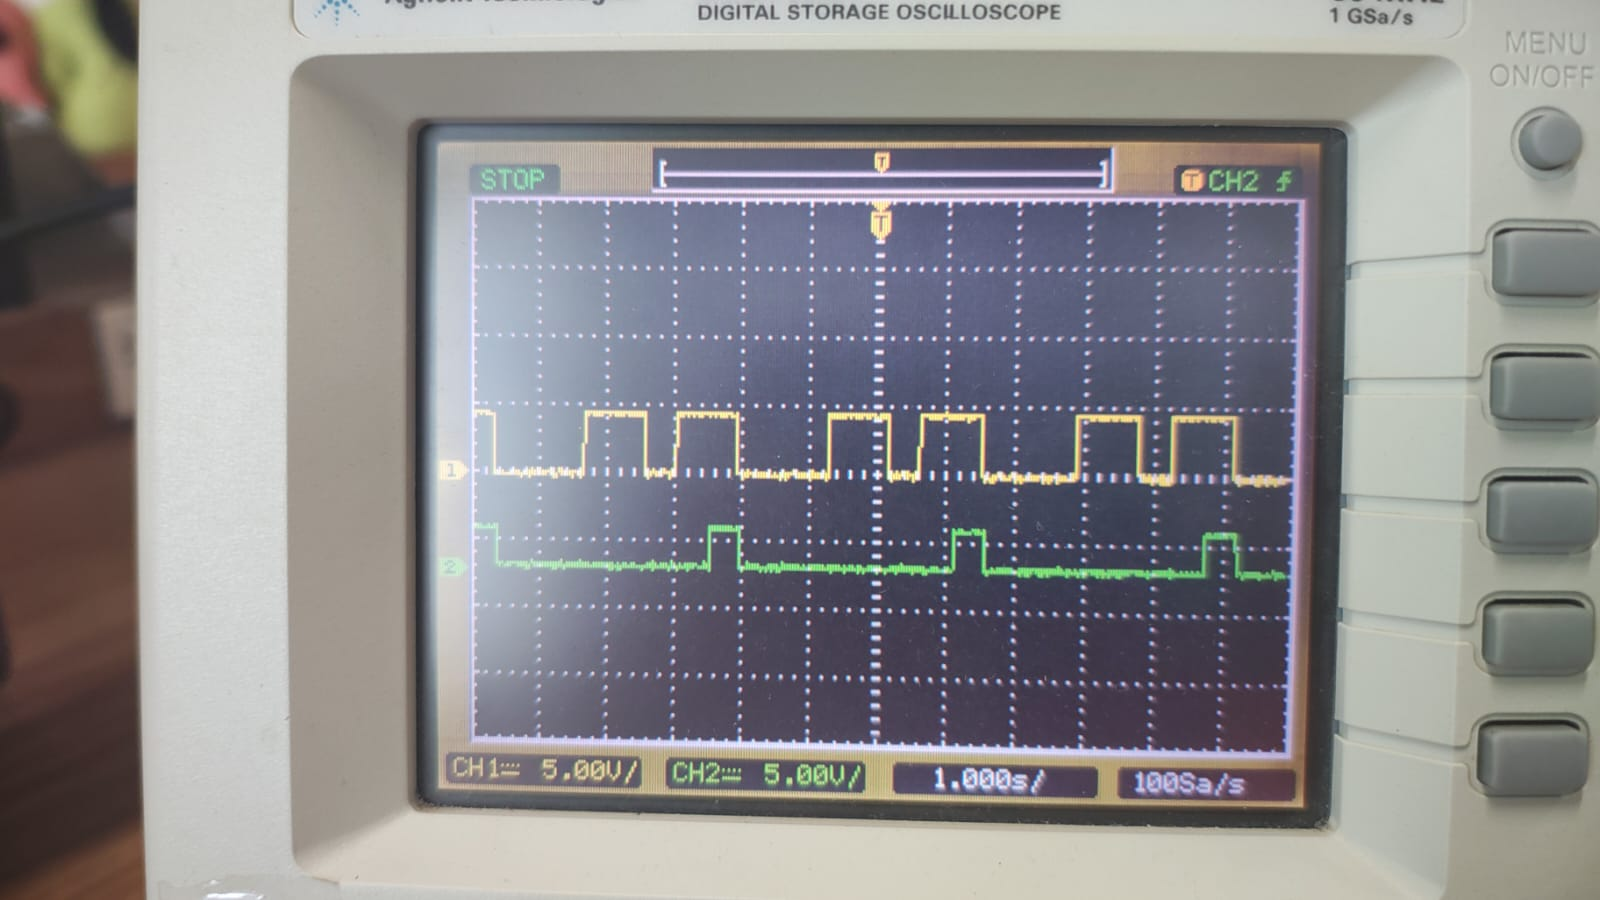
\includegraphics[width=0.95\textwidth]{figs/00011011.jpeg}
    \end{center}
    \caption{Oscilloscope reading for 00011011 repeated sequence}
\end{figure}

\begin{figure}
    \begin{center}
        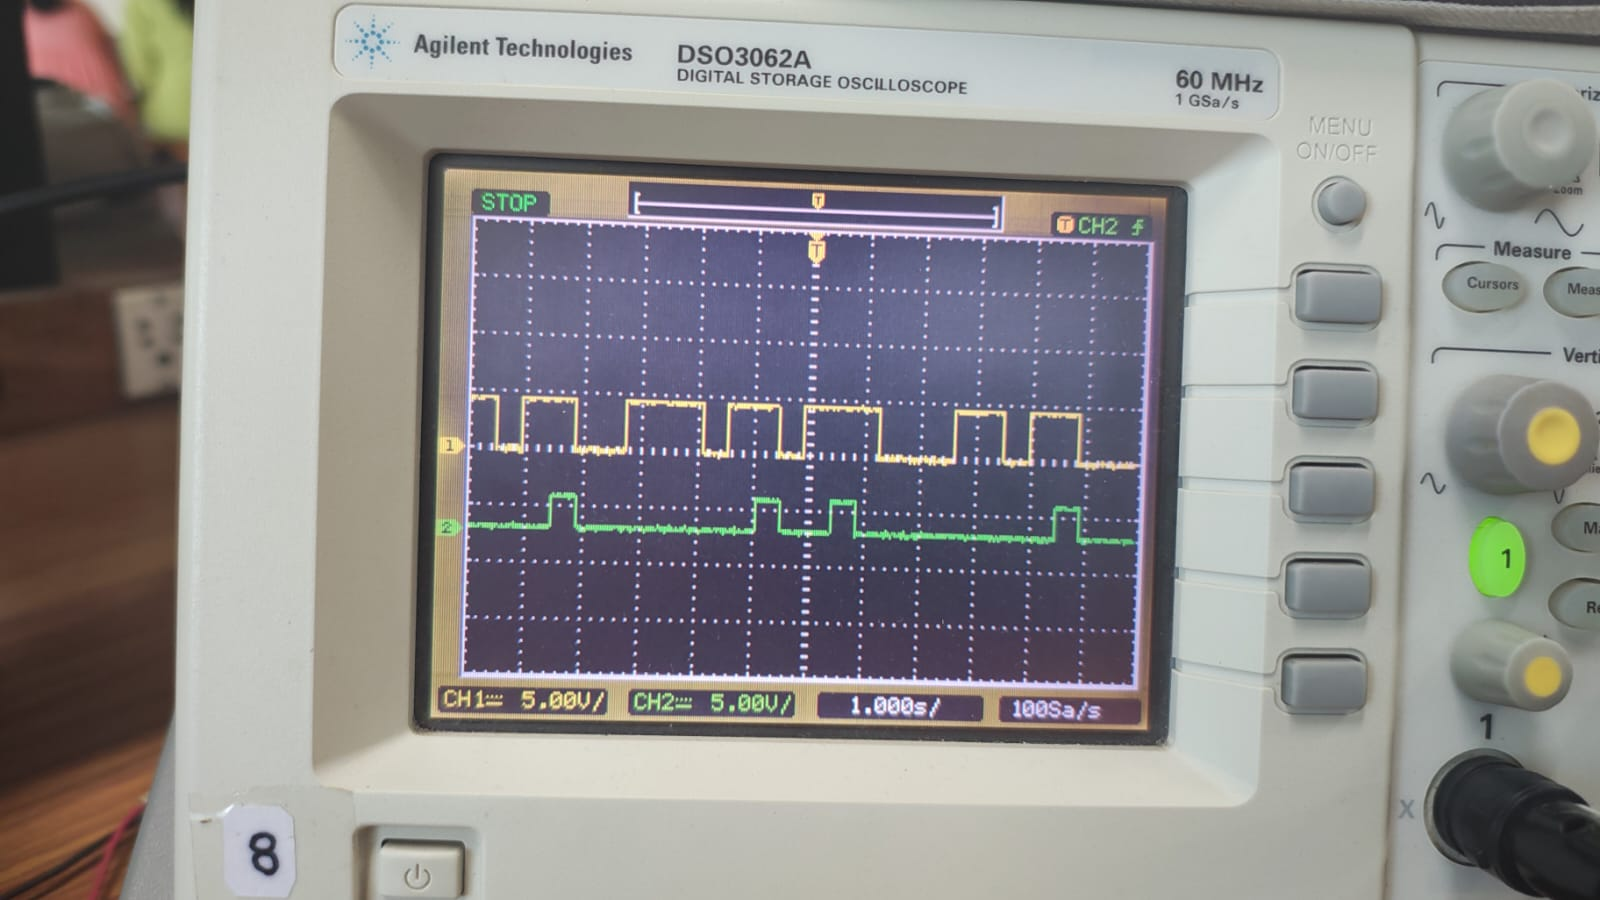
\includegraphics[width=0.95\textwidth]{figs/0001101100111011011100011011.jpeg}
    \end{center}
    \caption{Oscilloscope reading for 0001101100111011011100011011 repeated sequence}
\end{figure}

\begin{figure}
    \begin{center}
        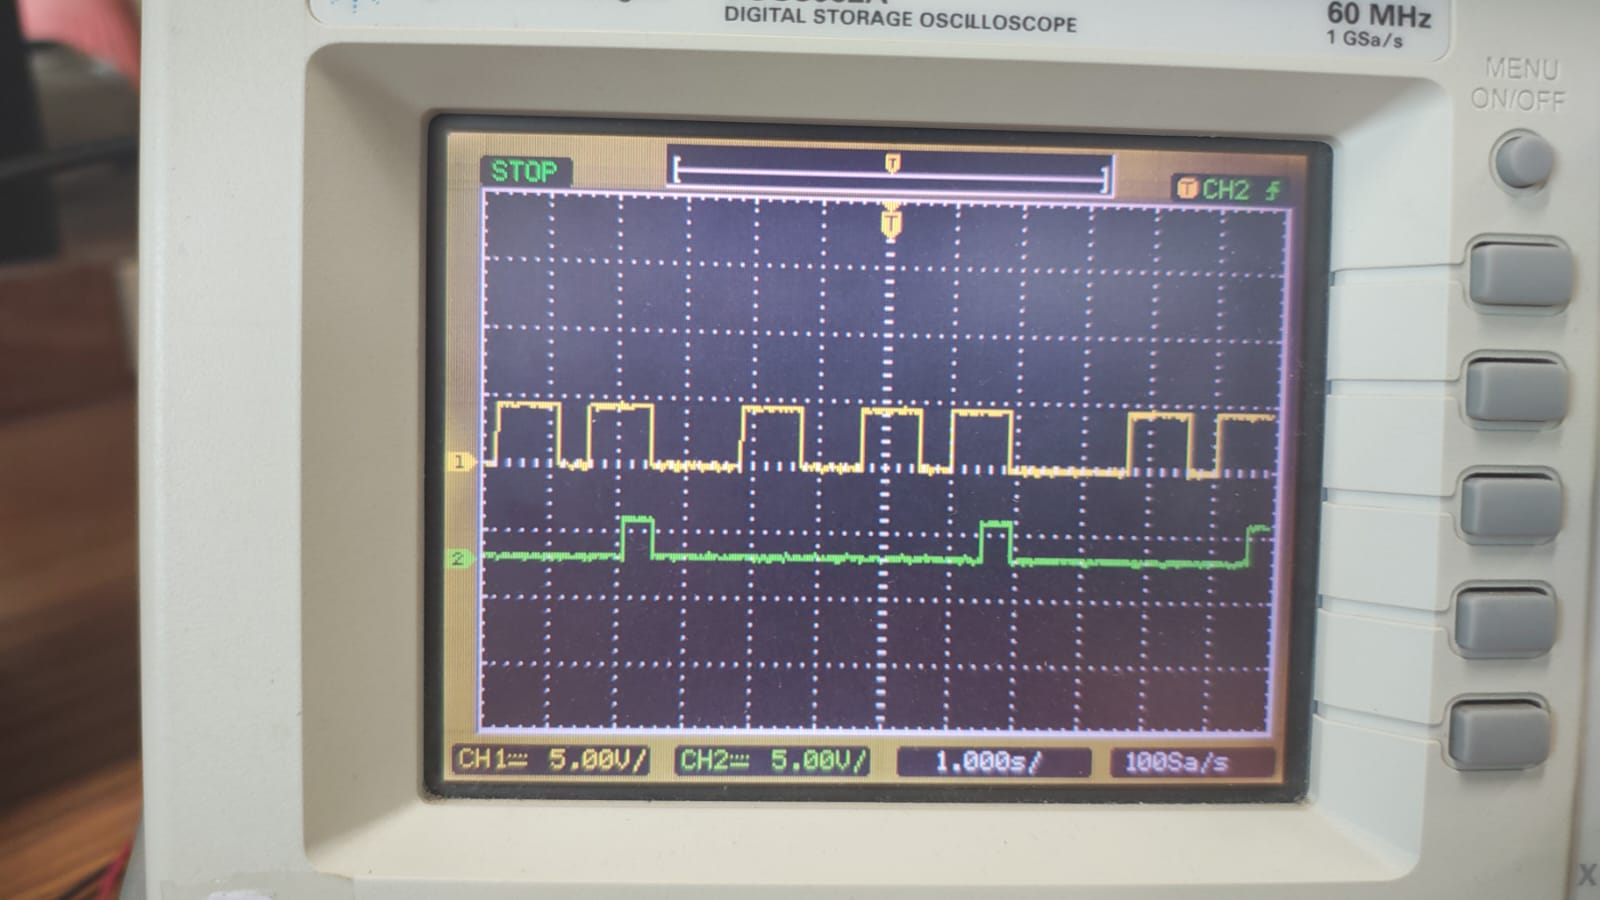
\includegraphics[width=0.95\textwidth]{figs/001101100001101100011.jpeg}
    \end{center}
    \caption{Oscilloscope reading for 001101100001101100011 repeated sequence}
\end{figure}

\begin{figure}
    \begin{center}
        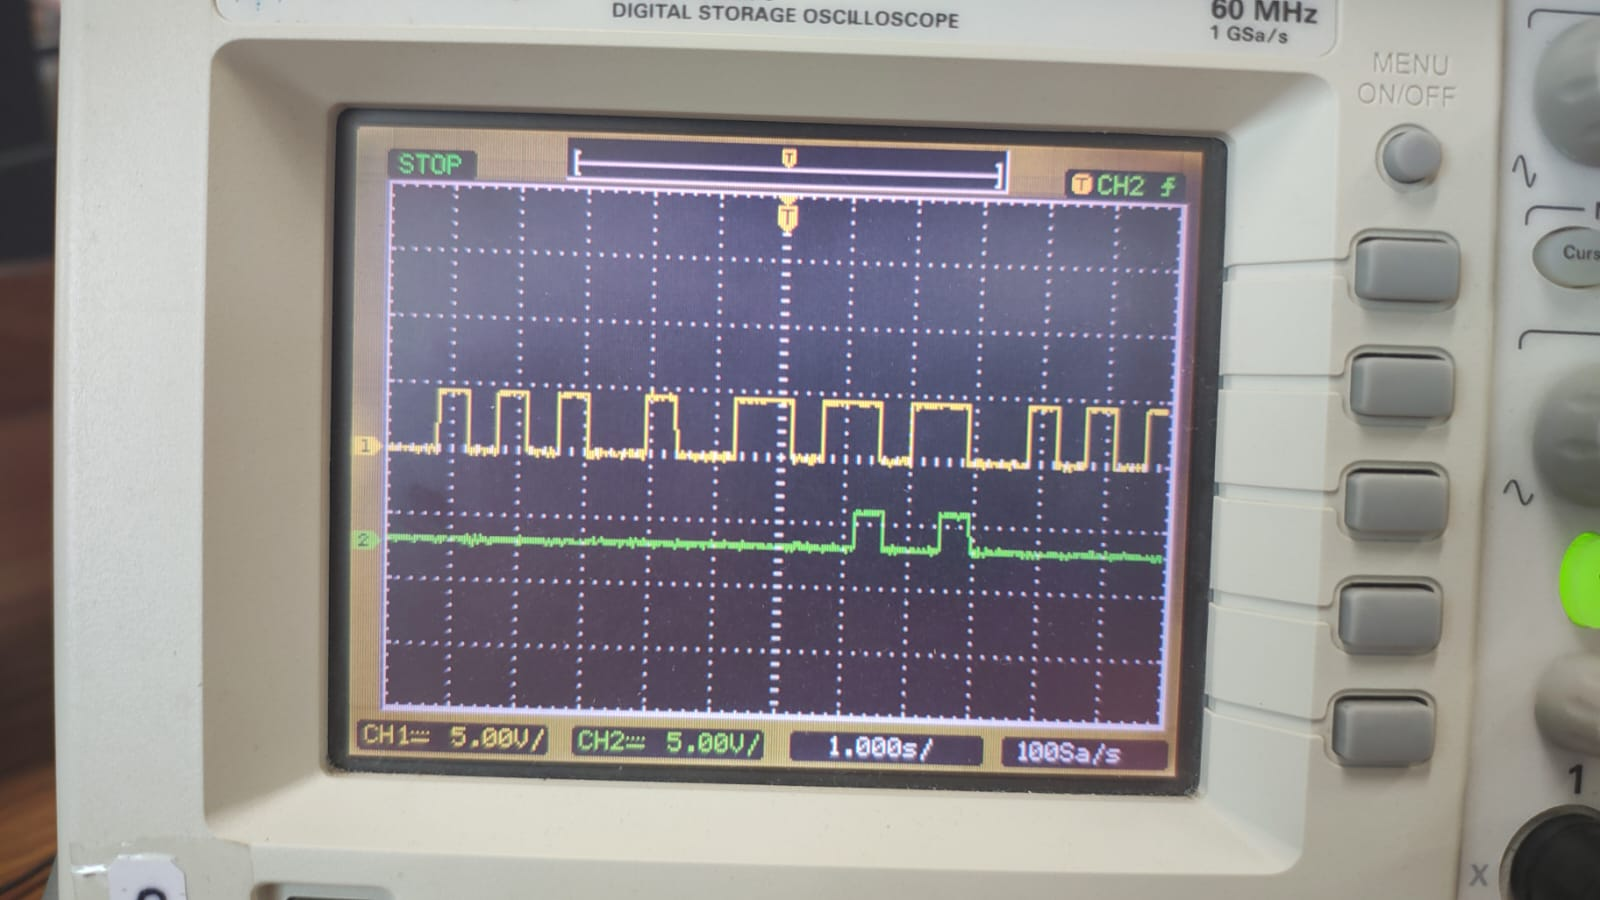
\includegraphics[width=0.95\textwidth]{figs/00110110110010101001.jpeg}
    \end{center}
    \caption{Oscilloscope reading for 00110110110010101001 repeated sequence}
\end{figure}

\begin{figure}
    \begin{center}
        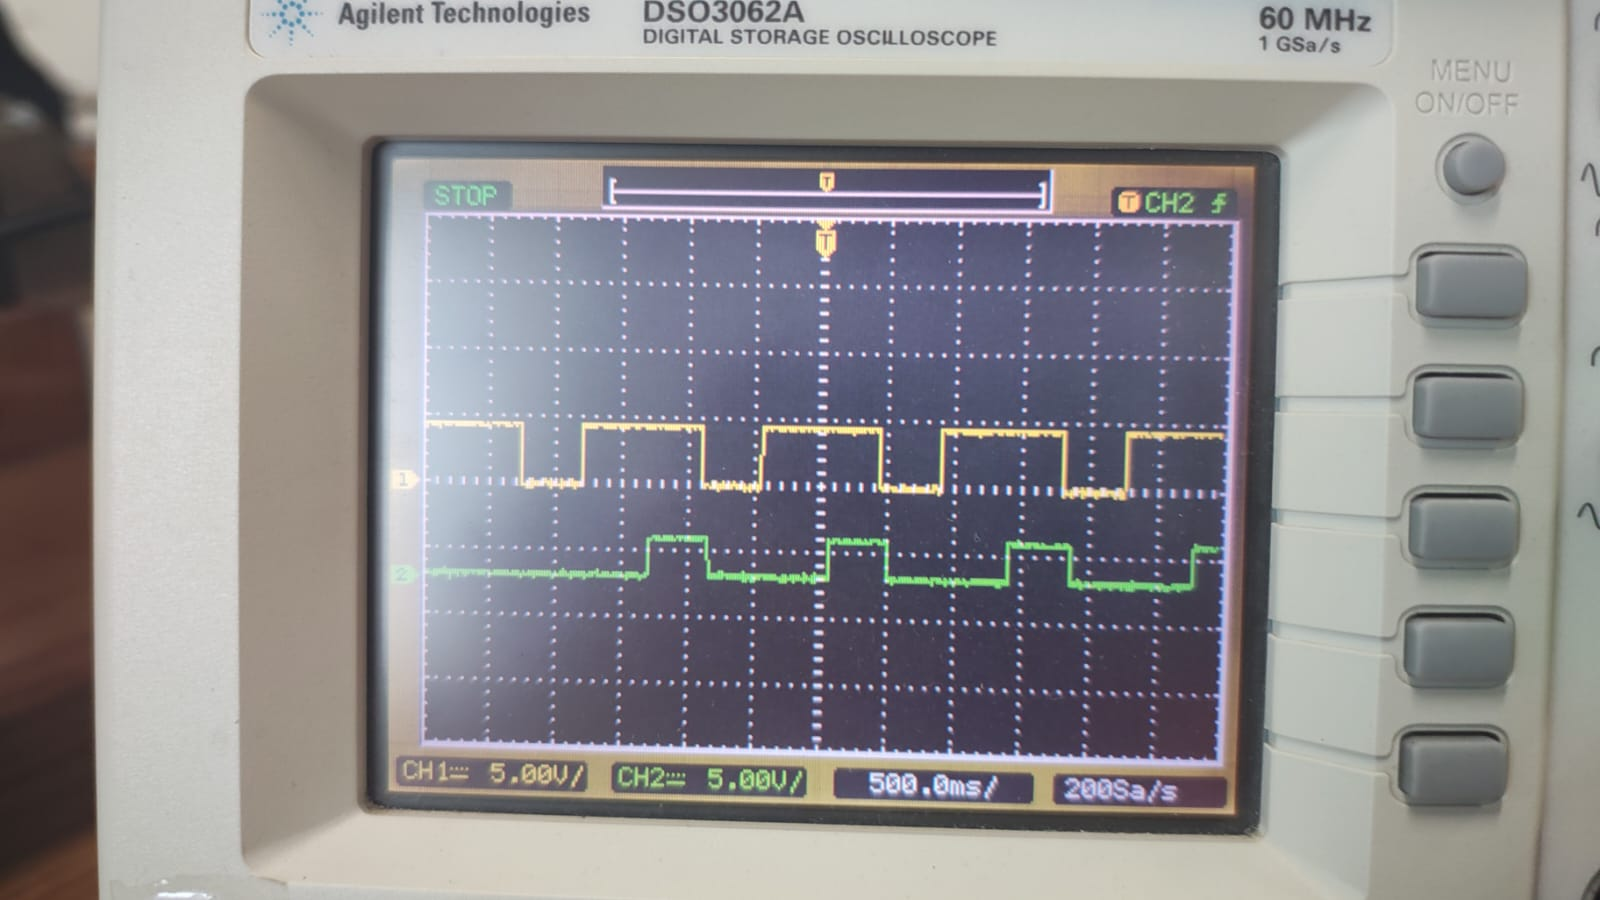
\includegraphics[width=0.95\textwidth]{figs/011011.jpeg}
    \end{center}
    \caption{Oscilloscope reading for 011011 repeated sequence}
\end{figure}

\begin{figure}
    \begin{center}
        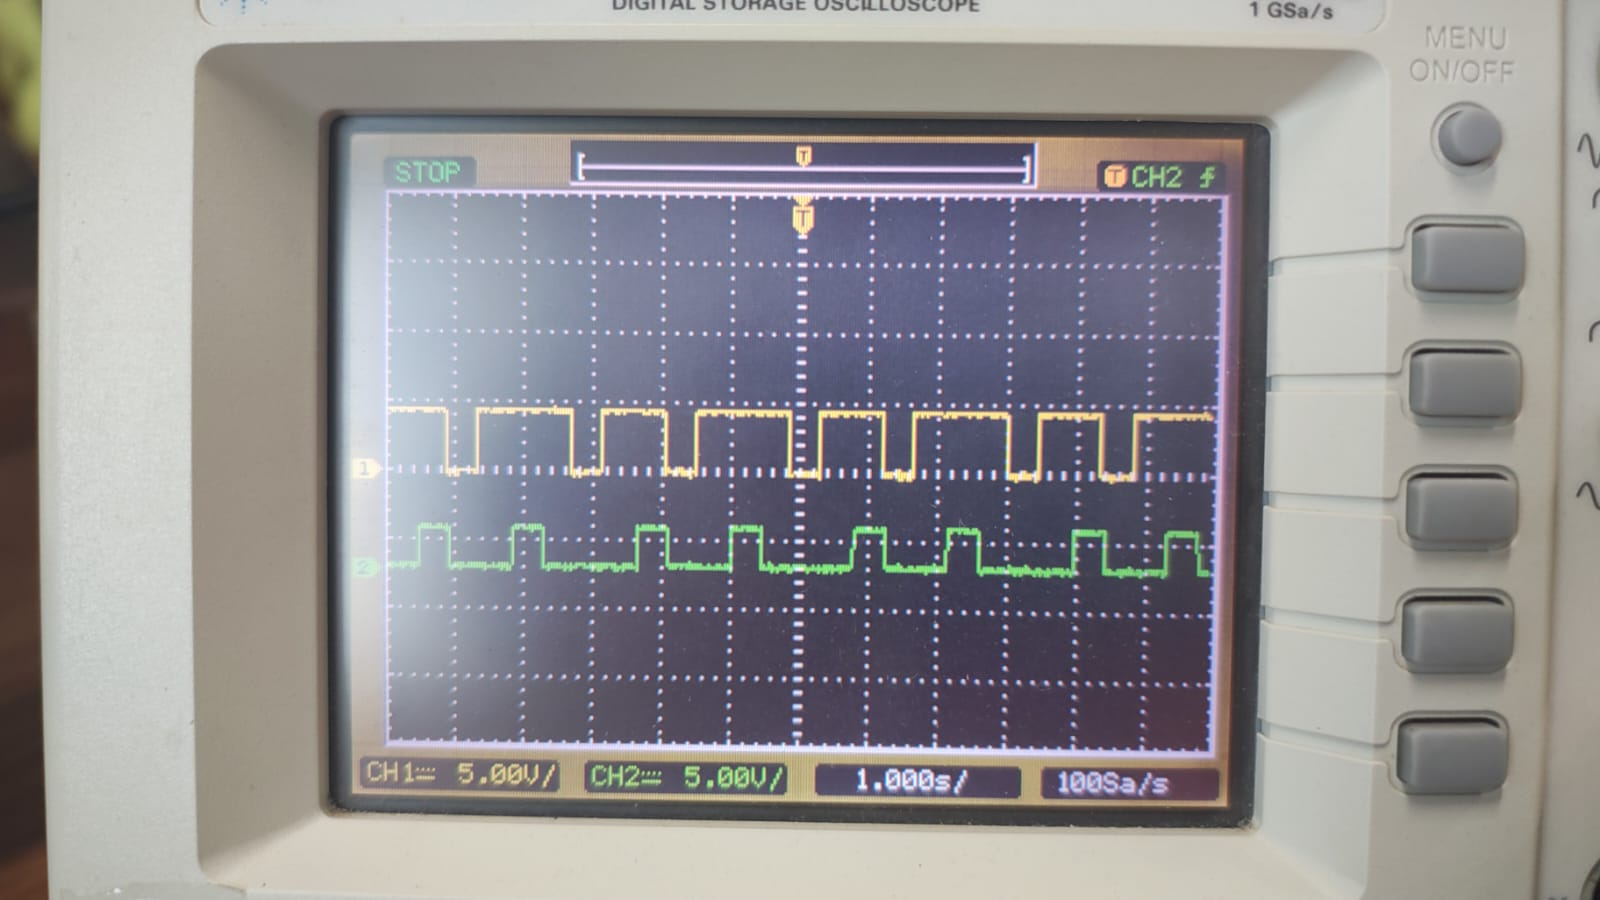
\includegraphics[width=0.95\textwidth]{figs/1011011.jpeg}
    \end{center}
    \caption{Oscilloscope reading for 1011011 repeated sequence}
\end{figure}
\FloatBarrier

\section{Circuit Picture and Video of Working}
Video can be downloaded at \href{https://github.com/AbhimanyuKoushik/EE1200/blob/main/Lab9/figs/video.mp4}{\textbf{here}}.
\begin{figure}[!ht]
    %\begin{center}
        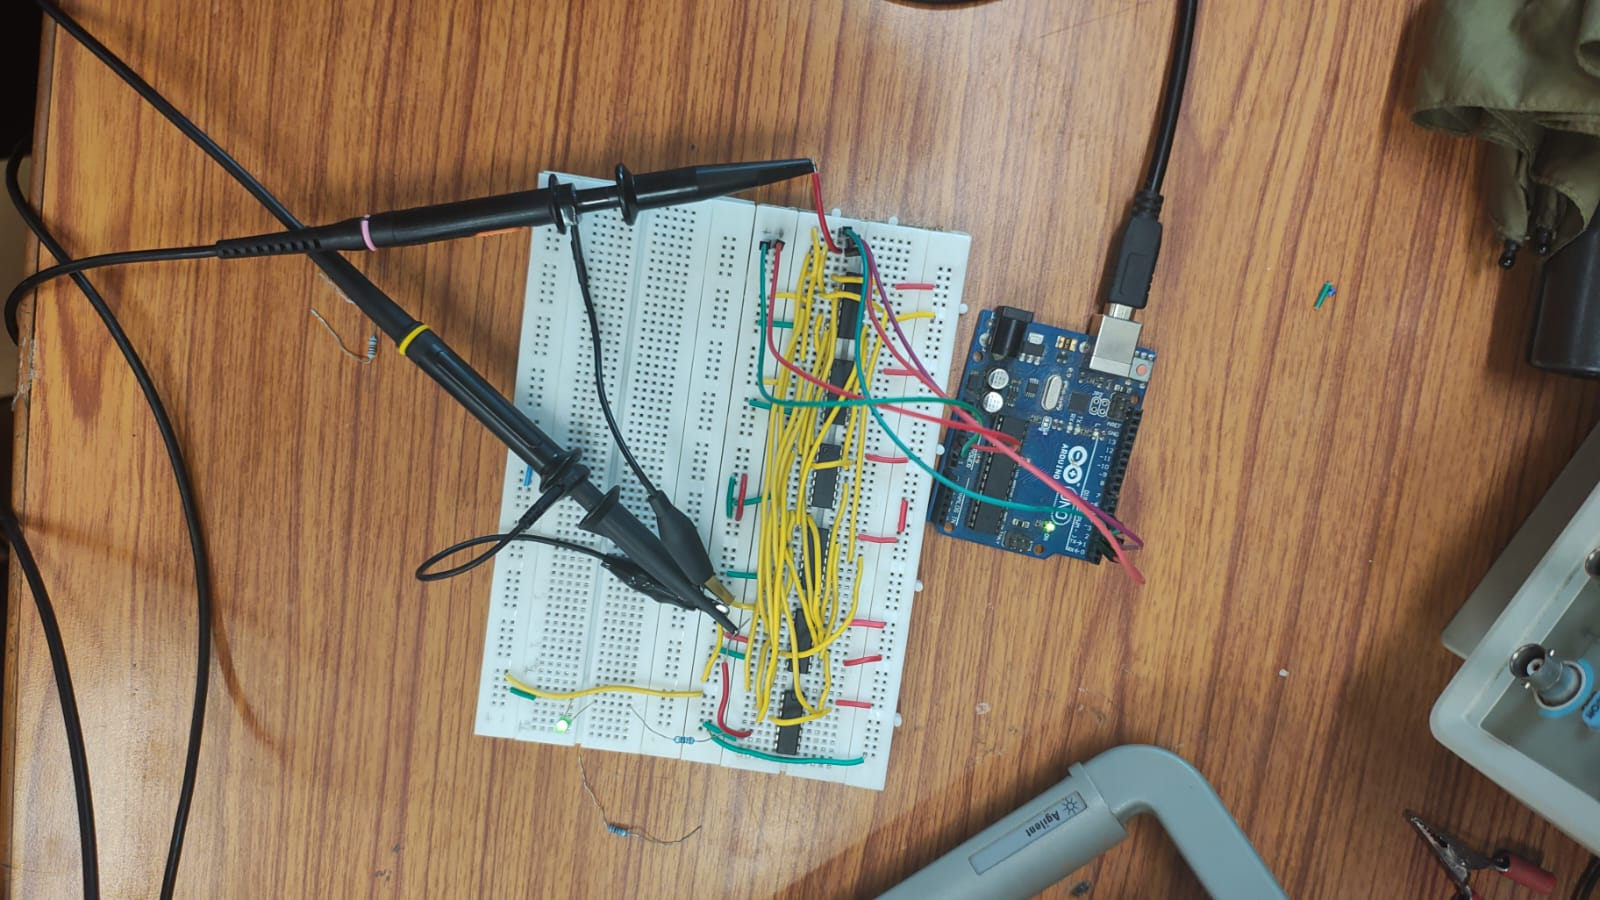
\includegraphics[width=0.95\textwidth]{figs/circuit3.jpeg}
    %\end{center}
    \caption{Circuit Picture}
\end{figure}

\section{Conclusion}

The Moore machine-based sequence detector for the "11011" pattern was successfully designed and implemented using D flip-flops (7474 ICs). The circuit correctly identified all occurrences of the target sequence in the input stream, including overlapping sequences.

\end{document}
